\documentclass{article}

\usepackage[utf8]{inputenc}
\usepackage{natbib}

\usepackage{graphicx}
\usepackage[section]{placeins}
\usepackage{fullpage}
\usepackage{todonotes}

\usepackage{amsmath}
\usepackage{amssymb}
\usepackage{bbold}
\usepackage{mathrsfs}

\usepackage{algorithm}
\usepackage[noend]{algorithmic} 

\DeclareMathOperator{\Tr}{Tr}
\DeclareMathOperator{\cst}{cst}
\DeclareMathOperator{\Gram}{Gram}
\DeclareMathOperator{\R}{\mathbb{R}}
\DeclareMathOperator{\E}{\mathbf{E}}
\DeclareMathOperator{\Y}{\mathcal{Y}}
\DeclareMathOperator*{\argmax}{arg\,max}
\DeclareMathOperator*{\argmin}{arg\,min}

\title{Stochastic Dual Coordinate Ascent \\ for \\ Conditional Random Fields}
\author{R\'emi LE PRIOL}
\date{\today}

\begin{document}

\maketitle

\section*{Introduction}

We apply the Stochastic Dual Coordinate Ascent (SDCA) algorithm to multi-class classification problems.
These problems are formulated as $l^2$ regularized negative log-likelihood minimization. 
We consider their dual : an entropy regularized centroid mean square error.
SDCA update one (block) coordinate at a time in the dual to raise the dual score.
  
First we focus on problems with a small number of classes for which SDCA's application is straight forward.
This is the framework of multinomial logistic regression.
Then we elaborate the theory for structured prediction problems.
In structured prediction, each class or label is a structured object.
There are too many of these objects to count them all.
More precisely we want to build a map from an input $x$ to a structured output $y$.
$y$ lives in a space that is finite but that is exponentially big in the size of $x$.
However we can use the structure over these $y$ to make the problem tractable.

In Conditional Random Fields (CRF), the labels distribution conditioned on the input is Markov with respect to an undirected graphical model (mathematician language) / Markov random field (computer scientist language). 
The dual problem's natural variables are the joint probabilities over all the potential labels.
We adapt the algorithm to the structure of the output by considering the marginals with respect to the cliques of that graph.

\section{Multiclass Logistic Regression}

\subsection{Linear Models}

We consider the following classical supervised setting.
We observe vector data $x_i$ in dimension d, associated to labels $y_i\in {1,..,K}$, for $i \in {1,..,n}$.
We note $X$ the design matrix of size n*d whose lines are the $x_i$.
We note Y the label matrix of size n*K whose line $Y_i$ is the one-hot encoding of the label $y_i$.
Given a new vector $x$, we want to predict what is the corresponding label $y$, or even better, a probability distribution over the classes ${1,..,K}$. 

The simpler models are linear classifiers : the probability for each class $y$ is proportional to $\exp(w_y^Tx)$, where the vectors $w_y$ are the parameters of the model.
In other word, we have one predictor per class, whose parameter is $w_y$.
The trick is that we will train these predictors jointly. 
We write $W$ the weight matrix whose lines are the $w_y$.
The closed formula for the conditional probability of y given x is thus :
\begin{equation}
	p(y|x;W) = \frac{\exp(w_y^Tx)}{\sum_{y=1}^K \exp(w_y^Tx)}
\end{equation}
With such models, we get polygonal classification boundaries, as shown in figure \ref{linear classification}.

For the sake of comparison, this is the same model as a neural network with no hidden layer, the input layer of size d, the output layer of size K, a weight matrix W of size K*d, and an exponential non-linearity.

\begin{figure}[ht]
	\label{linear classification}
	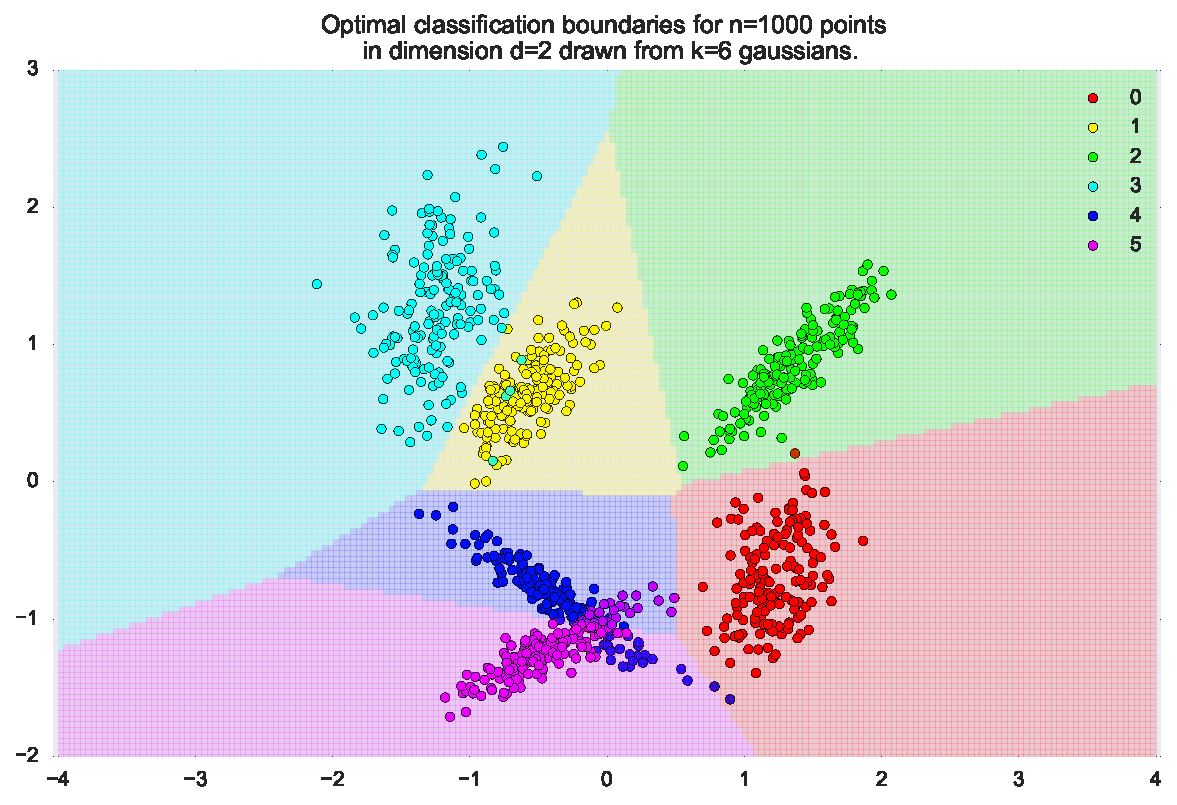
\includegraphics[width=\textwidth]{images/linear_classification.pdf}
	\caption{Optimal decision areas for the multinomial logistic regression.}
\end{figure}


 
 \subsection{Maximum Likelihood}
 
 The multinomial logistic regression is an optimization problem that we write to fit the model to the training data.
 It is the maximum likelihood estimator of the parameter W, regularized with the $l^2$ loss.
 We note $\lambda$ the regularization parameter, and $\mathscr{P}$ the primal function to optimize. 
 
 \begin{equation}
 	\min_{W \in \mathbb{R}^{K*d}} \mathscr{P}(W) = \frac{\lambda}{2}\sum_{y=1}^K  \|w_y\|_2^2 - \frac{1}{n} \sum_{i=1}^n \log p(y_i|x_i;W)
 \end{equation}
 
We further abbreviate $\|W\|^2 = \sum_{y=1}^K  \|w_y\|_2^2\|$ considering the Frobenius norm of $W$.
We also expand the expression of the conditional probability to get the classical formulation of the logistic regression problem.
We note $\Tr(Z)$ the trace of the matrix Z.

\begin{equation}
	\label{primal}
	\min_{W \in \mathbb{R}^{K*d}} \frac{\lambda}{2}\|W\|^2 + \frac{1}{n} \sum_{i=1}^n \log \bigg(\sum_y \exp(w_y^Tx_i)\bigg) - w_{y_i}^Tx_i 
\end{equation} 

We can write this problem in a more vectorial form by noting the log-partition function (the log-sum-exp) $\phi(z) = \log \big(\sum_{y=1}^K \exp(z_y)\big)$, and by introducing binary encoding of the ground truth Y. 

\begin{equation}
	\label{primal}
	\min_{W \in \mathbb{R}^{K*d}} \frac{\lambda}{2}\|W\|^2 + \frac{1}{n} \sum_{i=1}^n \phi(Wx_i) - \frac{1}{n}\Tr(Y W X^T) 
\end{equation} 

This is a convex problem in W.
Indeed the log-sum-exp is a convex function, as can be seen by verifying that it's Hessian is a semi-definite positive matrix.
The $l^2$ regularization guarantees that the function we are optimizing is at least $\lambda$ strongly convex. 

Let's notice that the gradient of the log-partition function evaluated in $Wx$ is the conditional probability vector of the classes given x : $\nabla\phi(Wx) = (p(y|x;W))_{y\in {1,..,K}}$.
This will prove useful in the following.

\subsection{Dual Formulation}

As any convex problem, the logistic regression admits dual formulations.
In this case, as the problem is unconstrained, these duals are called Fenchel duals.
We are given a splitting of the initial function to optimize in the form $f(x) + g(Ax)$ with x a vector, A a matrix, f and g two convex functions.
We note $f^*$ and $g^*$ the Fenchel duals of $f$ and $g$ respectively.
For simplicity, we do not write down the definition domains of these functions.
The Fenchel dual associated to this problem is derived as follows :
\begin{align*}
	 \min_x \ f(x) + g(Ax) & = \min_x \ \max_z z^Tx - f^*(z) + \max_y y^T A x - g*(y) \\
	 	& \geq \max_{z, y} \  \min_x x^T(z + A^T y) - f*(z) - g*(y) \\
		& =  - \min_y \   f^*(-A^Ty) + g^*(y) \quad \textrm{if} \quad z=-A^T y \quad , -\infty \textrm{ otherwise.}\\
\end{align*}

Importantly enough, each splitting of the function in arbitrary pairs of convex functions can yield a different dual formulation.
For the logistic regression, rather than splitting the function in this canonical form, we get the dual formulation by injecting the equation $f(x) = \max_y x^T y - f^*(y)$ for the $l^2$ regularization and each of the log-sum-exp.
We then get the canonical dual problem : \todo{Should I derive the dual formulation here?}
\begin{equation}
	\max_{\alpha\in \Delta_K^n} \mathscr{D}(\alpha) = -\frac{\lambda}{2} \|W(\alpha)\|^2 + \frac{1}{n} \sum_{i=1}^n H(\alpha_i)
\end{equation}
where $\Delta_K$ is the simplex of dimension K, meaning that $\alpha$ is a n*K matrix whose lines live in the simplex.
H is the entropy of dimension K : $H(\alpha_i) := - \sum_y \alpha_i(y) \log(\alpha_i(y)$.
$\alpha$ should be interpreted as a distribution of weight on the different classes for each example.
What we call the primal parameters associated to alpha is defined by the equation :
\begin{equation}
	w_y(\alpha) := \frac{1}{\lambda n} \sum_i (\mathbb{1}_{y=y_i} - \alpha_i(y)) x_i 
\end{equation}
We can also write it with matrices : 
\begin{equation}
	\label{primal to dual}
	W(\alpha) = \frac{1}{\lambda n} (Y - \alpha)^T X 
\end{equation}
Or we can separate the influence of each example i through $\alpha_i$ on the resulting vector W :
\begin{equation}
	\label{individual w}
	W(\alpha) = \frac{1}{n} \sum_i W_i(\alpha_i) \quad \textrm{where} \quad W_i(\alpha_i) := \frac{1}{\lambda} (Y_i - \alpha_i) x_i^T
\end{equation}

This equation correspond to an optimality condition that appears when one derives the dual formulation.
Similarly, when we derive the primal problem from the dual problem, we get the optimality condition :
\begin{equation}
	\label{dual to primal}
	\alpha_i(W) = \nabla\phi(Wx_i) = p(y_i|x_i;W)
\end{equation}
This optimality condition means that at the optimum, the dual problem and the primal problem give the same distribution on the classes of each instance i.

As the primal problem is unconstrained, strong duality holds for this problem.
Thus the optimum points $W^*$ and $\alpha^*$ verify equality in both equations \ref{primal to dual} and \ref{dual to primal}.
See  \verb https://en.wikipedia.org/wiki/Fenchel%27s_duality_theorem \verb  for real conditions.


\subsection{Stochastic Dual Coordinate Ascent}
As the name suggests the SDCA algorithm updates each line of the matrix $\alpha$ at a time.
At each time step, one $i\in{1,..n}$ is picked at random.
Then $\alpha_i$, which lives in the simplex, is updated so as to maximize the dual objective.
Finding the optimal update for $\alpha_i$ is a constrained optimization problem in dimension K, which can be itself difficult. 
In his 2013 paper \cite{shalev-shwartz_accelerated_2013-1}, Shalev-Shwartz analyzes the brilliant idea of updating $\alpha_i$ in the direction of a subgradient of the primal loss $\nabla\phi(W(\alpha)x_i)$.
This is also what $\alpha_i$ should be equal to : $\alpha_i(W(\alpha))$.
One can then either take steps of fixed size in the ascent direction $d_i := \alpha_i(W(\alpha)) - \alpha_i$, or can perform a line search on the segment between $\alpha_i$ and $\alpha_i(W(\alpha))$.
\todo{insert drawing of the segment in the simplex.}

\todo{pseudo code of my algorithm.
Specify why I can keep W as well as alpha.
What are the memory and time cost of SDCA.
How does it compare with SAG etc...}
% $W^{(t+1)} = W^{(t)} + W_i(\alpha_i^{(t+1)}) - W_i(\alpha_i^{(t)})$. 


\paragraph{Line search }: the function of the step size we want to optimize is 

\begin{equation}
	\label{line search 1}
	f_i(\gamma) = -\frac{\lambda n}{2} \|W(\alpha + \gamma d_{[i]})\|^2 + H(\alpha_i + \gamma d_i) + \cst
\end{equation}
where he $d_{[i]}$ is the matrix n*K whose line i is $d_i$ and where the rest is 0.
The first term is a quadratic function in $\gamma$.
It can be expanded with equation \ref{primal to dual}.
We note $\beta = Y - \alpha$ the difference between the ground truth and the dual estimation. 

\begin{align*}
	-\frac{\lambda n}{2} \|W(\alpha + \gamma d_{[i]})\|_F^2 & = -\frac{\lambda n}{2} \Tr(W(\alpha + \gamma d_{[i]}) W(\alpha + \gamma d_{[i]})^T) \\
	& = -\frac{1}{2\lambda n} \Tr((\beta - \gamma d_{[i]})^T X X^T (\beta - \gamma d_{[i]})) \\
	& = -\frac{1}{2\lambda n} \bigg[ \Tr(\beta X X^T \beta) - 2\gamma\Tr(\beta^TXX^Td_{[i]}) + \gamma^2 \Tr(d_{[i]}^TXX^Td_{[i]})\bigg] \\
	& = -\frac{\lambda n}{2} \|W(\alpha)\|_F^2 + \gamma\Tr(W(\alpha)X^Td_{[i]}) - \gamma^2 \frac{\|d_i\|^2 \|x_i\|^2}{2\lambda n} \\
	& = -\frac{\lambda n}{2} \|W(\alpha)\|_F^2 + \gamma \ d_i^T W(\alpha) x_i - \gamma^2 \frac{\|d_i\|^2 \|x_i\|^2}{2\lambda n}
\end{align*}

We expand the first term  of \ref{line search 1} with the formulation above to highlight the quadratic dependency on $\gamma$.

\begin{equation}
	f_i(\gamma) = - \gamma^2 \frac{\|d_i\|^2 \|x_i\|^2}{2\lambda n^2} + \gamma \ d_i^T W(\alpha) x_i + H(\alpha_i + \gamma d_i) + \cst
\end{equation} 

This is indeed a concave function.
Its derivatives are as follow.
\begin{equation}
	f_i'(\gamma) = - \gamma \frac{\|d_i\|^2 \|x_i\|^2}{\lambda n^2} + d_i^T W(\alpha) x_i- \sum_y d_i \log(\alpha_i + \gamma d_i)
\end{equation}
\begin{equation}
	f_i''(\gamma) = - \frac{\|d_i\|^2 \|x_i\|^2}{\lambda n^2} - \sum_y \frac{d_i^2}{\alpha_i + \gamma d_i}
\end{equation}

We can find the $2\epsilon$-approximate maximum of such a function defined on [0,1] by looking at the $\epsilon$-approximate root of its derivative on $[\epsilon,1-\epsilon]$.
This can be done with a stabilized Newton method for instance, as described in the section 9-4 of the book \cite{press_numerical_1992}.


\subsection{Duality Gap and Non-Uniform Sampling}
As SDCA keeps track of both a dual variable $\alpha$ and a primal variable $W(\alpha)$, abbreviated $W$ in the following, we can evaluate the duality gap between the primal problem evaluated in $W$ and the dual problem evaluated in $\alpha$. 
\begin{align*}
	g(\alpha,W) & = \mathscr{P}(W) - \mathscr{D}(\alpha)\\
	& = \lambda \|W\|^2 	+\frac{1}{n}\sum_{i=1}^n \big[ \phi(Wx_i) - H(\alpha_i)\big] - \frac{1}{n}\Tr(Y W X^T) \\
	& = \frac{1}{n}\sum_{i=1}^n \big[ \lambda \langle W_i(\alpha_i),W\rangle + \phi(Wx_i) - H(\alpha_i) - Y_i^T W x_i\big] \quad \textrm{where} \quad W_i(\alpha_i) := \frac{1}{\lambda} (Y_i - \alpha_i) x_i^T \\
	& = \frac{1}{n}\sum_{i=1}^n \big[ \Tr(x_i (Y_i-\alpha_i)^T W) + \phi(Wx_i) - Y_i W x_i - H(\alpha_i)\big]\\
	& = \frac{1}{n}\sum_{i=1}^n \big[\phi(Wx_i) - H(\alpha_i) - \alpha_i^T W x_i\big]
\end{align*}

If we note $s_i=Wx_i$ the score given by our primal model to the different classes on the example i, the total duality gap can then be written as the mean of individual gaps : 
\begin{equation}
	g_i(\alpha_i,s_i) = \phi(s_i) - H(\alpha_i) - \langle\alpha_i, s_i\rangle
\end{equation}
$g_i$ is really a duality gap.
The log-partition $\phi$ and the entropy $-H$ are convex conjugates.
Consequently, $g_i$ is the Fenchel duality gap between $\phi(s_i)$ and $H(\alpha_i)$.
It is always positive and  it represents the sub-optimality we have on the datapoint i.
It can also be expressed as the Kullback-Leibler divergence between the dual distribution $\alpha_i$ and the primal distribution $\nabla_i := \nabla\phi(s_i) = \exp(s_i - \phi(s_i))$.
Indeed $\langle\alpha_i, s_i\rangle$ becomes $\langle\alpha_i, \log(\nabla_i)\rangle + \phi(s_i)\langle\alpha_i, \mathbb{1}\rangle = \E_{\alpha_i}[log(\nabla_i)] + \phi(s_i)$
\begin{equation}
	g_i(\alpha_i,\nabla_i) = D_{KL}(\alpha_i || \nabla_i)
\end{equation}

In the article \cite{osokin_minding_2016}, the author apply a non-unform sampling scheme on the algorithm Block Coordinate Frank-Wolfe \cite{lacoste-julien_block-coordinate_2012}. 
Their scheme is to sample proportionally to past-estimates of the individual duality gaps.
In SDCA, we have access to duality gap $g_i$ if we pick the element i for almost no extra cost.
Indeed each step involves computing $s_i = W x_i$ to get $\alpha_i(W(\alpha))=\nabla\phi(s_i)$.
So we can get $\phi(s_i)$ in time $O(K)$.
$H(\alpha_i)$ is already computed during the line search, and is done in $O(K)$ as well.
Finally the scalar product $\langle\alpha_i, s_i\rangle$ has to be computed for a similar cost $O(K)$.  


\subsection{Results}

SDCA gives proper results on synthetic gaussian mixtures datasets. 
\begin{figure}[ht]
	\label{gmm results}
	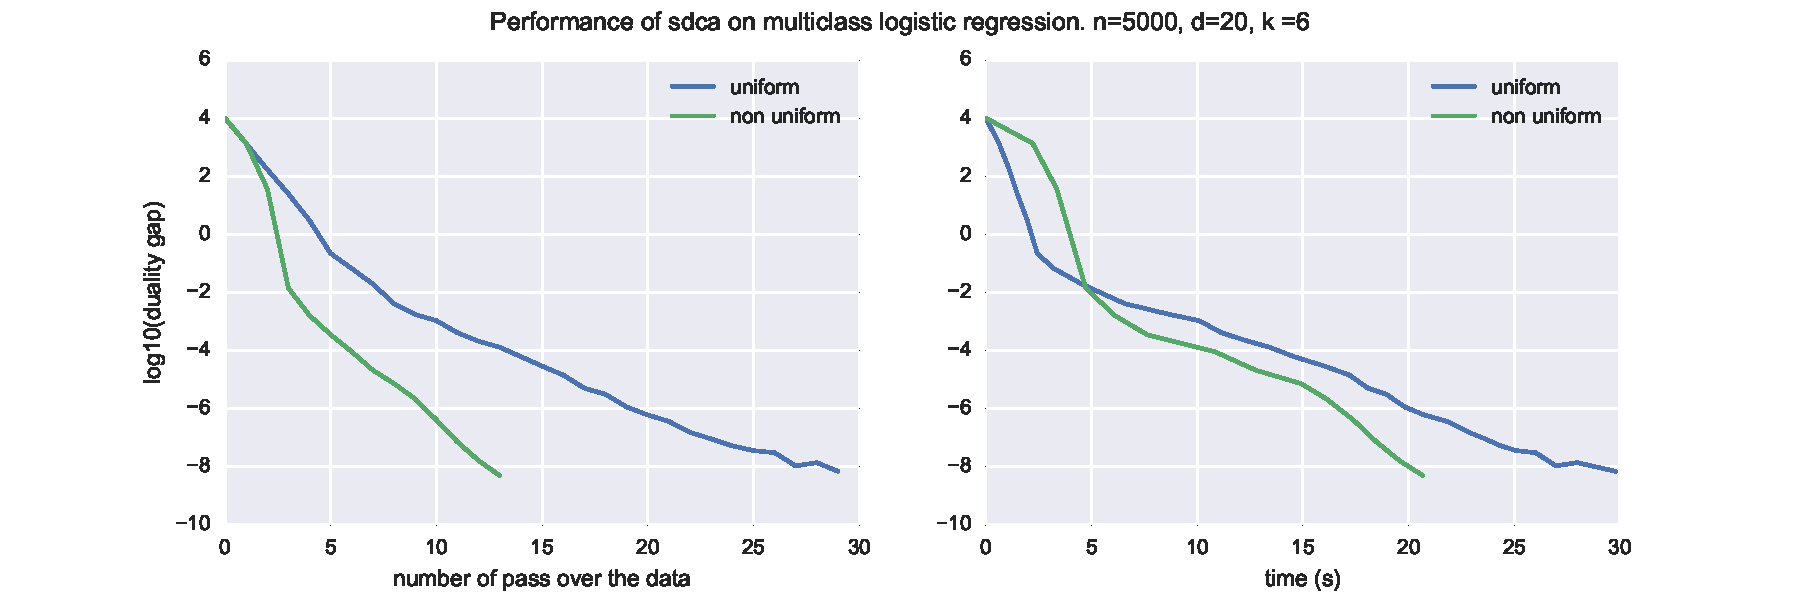
\includegraphics[width=\textwidth]{images/nonuniform_is_better.pdf}
	\caption{Comparison of the performance of various methods on a synthetic Gaussian mixture dataset.}
\end{figure}

\todo{Comparison with the other non-uniform sampling method on a real dataset?}


%%%%%%%%%%%%%%%%%%%%%%%%%%%%%%%%%%%%%%%%%%%%%%%%%%%%%%%%%%%
% CRF 
%%%%%%%%%%%%%%%%%%%%%%%%%%%%%%%%%%%%%%%%%%%%%%%%%%%%%%%%%%%
\clearpage
\section{Conditional Random Fields}

\subsection{Structured Prediction}

Structured prediction is a sub genre of multi-class classification problem.
The particularity is that we have structure information about the class themselves.
For instance we would like to identify words from images of letters, and we know that there is a chain structure on these letters (OCR\todo{put citation   here}).
Or we could parse written mathematical expressions and we know that there is a natural tree structure on these expressions.
Another typical instance is semantic segmentation in images : we know a priori that boundaries between objects should be sharp and that objects are usually connected areas.
Let's write x for the input data point and y for the output class that lives in $\Y_x$.
We index $x$ to $\Y$ because the space of classes can depend on $x$.
For instance, the word we predict will have as many letters as we have images, and the semantic segmentation will be an image of the same size as the input image. 

Compared to standard multi-class classification, we need to exploit the structure because the output space $\Y_x$ has a size that is typically exponential in the size of the input x.
A brute force approach listing the probabilities for each class to take the max is thus intractable.
The structure generally allows us to explore the space of classes in a clever way, to compute the mode of this distribution or the marginal probabilities on some part of the structure.
We call the algorithm that returns the mode the \textit{max oracle} and the one that returns the marginals the \textit{marginalization oracle}. 

Formally, for any pair (input, output) we want to define a structured score $s_w(x, y)$ parametrized by a vector w.
This score should represent the confidence that we have that the point x belongs to the class y through the equation $p(y|x ; w)\propto \exp(s_w(x, y))$.
Physically, the score  is thus the opposite of the energy of the state y for the system x. 
\begin{equation}
	\label{primal probability}
	p(y|x; w)=  \frac{e^{s_w(x, y)}}{\sum_{y'} e^{s_w(x, y')}}
\end{equation}

In the following, we assume that we have a feature extractor for pairs $x, y \mapsto F(x, y) \in \R^d$, either handcrafted or pre-trained.
Our score will be a linear combination of these features.
We call the parameter w \textit{the weights}.
\begin{equation}
	s_w(x, y) = \langle w, F(x, y) \rangle
\end{equation}

We consider output spaces specified by undirected graphical models, aka Markov Random Fields.
The output y is a random variable that factors over the graph $G=(V,E)$.
Formally, this means that the joint probability over y can be factorized into potentials over the maximal cliques of the graph.
We denote the $\mathcal{C}$ the set of maximal cliques of G, and $\mathcal{S}$ the set of separations between these cliques.

\begin{align*}
	p(y|x ; w) & \propto  \exp(s_w(x, y) \\
	& \propto \prod_{c\in \mathcal{C}} \exp(s_{w, c}(x, y_c))\\
	& \propto  \prod_{c\in \mathcal{C}} \exp(\langle w, F_c(x, y_c) \rangle) \\
	& \propto \exp( \langle w, \sum_{c\in \mathcal{C}} F_c(x, y_c) \rangle 
\end{align*}
We go from the second to the third line by assuming that the score of each clique is itself linear.
The consequence of these derivations is that if y factors over a graph, we want the features to be separable the same way :
\begin{equation}
	F(x, y) =  \sum_{c\in \mathcal{C}} F_c(x, y_c)
\end{equation}


\subsection{Maximum Likelihood}

We have a set of n pairs $(x_i, y_i) \in \mathcal{X} \times \Y_i$ independently sampled.
We also have a feature extractor that maps these pairs to $\R^d$.
This feature extractor is separable over graphs of the appropriate dimension corresponding to each $\Y_i$.
The Conditional Random Field model aims at maximizing the log-likelihood of the weights $w\in \R^d$ given these samples.
Once we have learnt the weights, we can predict the class of a new data point x by taking the mode of $p(y|x ; w)$.
The prediction function is thus $x \mapsto \hat{y} = h_w(x) = \argmax_{y\in \Y_x} s_w(x, y)$.
To avoid overfitting and to make the problem strongly convex, we penalize the squared $l^2$ norm of the weights.
The variational CRF problem is written below.

\begin{equation}
\min_{w\in\R^d} f(w) = \frac{\lambda}{2}\|w\|^2 - \frac{1}{n}   \sum_{i=1}^{n} \log(p(y_i|x_i; w))	
\end{equation}

Let's expand the probability term in this formula.
We define the corrected features $\psi_i(y)$ of a class y for the point i as the difference between the ground truth features and the features of $(x_i, y)$.
\begin{equation}
	\psi_i(y)) := F(x_i, y_i) - F(x_i, y)
\end{equation}
The negative log-likelihood then becomes the log-partition function (log-sum-exp) $\phi_i(z):=\log(\sum_{y\in \Y_i} e^{z(y)})$ over these features.
\begin{equation}
	- \log(p(y_i|x_i; w)) = \log \bigg ( \sum_{y \in \Y_i}  \exp(-w^T\psi_i(y)) \bigg ) = \phi_i(-A_i^Tw)	
\end{equation}
where $A_i$ \todo{Change the name of $A_i$ for a more typical one.
Idem for $\phi_i$} is the $d\times |\Y_i|$ matrix whose columns are the $\psi_i(y)$ for $y \in \Y_i$.
We index $i$ to $\phi_i$ because it affects the range of the sum.
The closed formulation of the CRF is thus :

\begin{equation}
\min_{w\in\R^d} f(w) = \frac{\lambda}{2}\|w\|^2 + \frac{1}{n}   \sum_{i=1}^{n} \phi_i(-A_i^Tw)	
\end{equation}


%%%%%%%%%%%%%%%%%%%%%%%%%%%%%%%%%%%%%%%%%%%%%%%%%%%%%%%%%%
\subsection{Dual Formulation}

We can derive a Fenchel dual to the CRF, as done in \todo{provide reference.}
\begin{equation}
	\max_{\alpha\in\Delta_{1} \times \dots \times \Delta_{n}} -\frac{\lambda}{2}\|w(\alpha)\| +\frac{1}{n} \sum_{i=1}^n H_i(\alpha_i)
\end{equation}
where $\Delta_i$ is the simplex of dimension $|\Y_i|$, meaning that $\alpha$ is a n*$|\Y_i|$ matrix whose lines live in the simplex, and $H_i$ is the entropy for distributions over $\Y_i$ : $H(\alpha_i) := - \sum_y \alpha_i(y) \log(\alpha_i(y)$.
To simplify the notation, we omit the domain of summation for y in the sum as it can be deduced from the context.
We define the \textit{dual weights} given by the optimality condition:
\begin{equation*}
	w(\alpha) = \frac{1}{\lambda n} \sum_i \sum_y \alpha_i(y) \psi_i(y) 
\end{equation*}
At the dual optimum $\alpha^*$, $w(\alpha^*)$ is optimum for the primal problem.
This formula can be written in a number of ways, each time outlining some property.
\begin{align}
	w(\alpha) & = \frac{1}{\lambda n} A \alpha \label{linear combination of probabilities} \\
	 & = \frac{1}{\lambda} \E_{i} [ \E_{y \sim \alpha_i} [\psi_i(y)]] \label{mean of the corrected features} \\
	 & =   \frac{1}{\lambda} \E_{i} [F(x_i, y_i)] - \frac{1}{\lambda} \E_{i} [ \E_{y \sim \alpha_i} [F(x_i, y)]]
	 \label{difference between ground truth and dual weights}
\end{align}
where A is the horizontal concatenation of the $A_i$.
It is a matrix of size $d \times \sum_i |\Y_i|$.
The expectations over i assume i is uniform random variable taking its values between 1 and n. 

\paragraph{Interpretation :} The primal problem is a regularized maximization of the likelihood of w. 
In the dual problem, we control directly the probabilities given to each class on the training samples.
There is two conflicting terms.
The first one aims at minimizing the size of the centroid of the corrected features.
Since $\psi_i(y_i)=0$, it is minimal for the empirical distribution.
The second term aims at maximizing the entropy of this distribution.
It pushes the $\alpha_i$ towards a more uniform distribution.
Thus the role of the terms is the inverse of the primal model : the data fitting term is on the left.
It is the squared distance between the centroid of the ground truth features and the centroids predicted by the dual model.
The entropy on the right is the regularization. 

We can also derive the primal problem from the dual problem.
We then get another optimality condition $\alpha(w^*) = \alpha*$ where $\alpha(w)$ is the density on the training set defined by the weights w in equation \ref{primal probability}.

\begin{equation}
	\forall i, \alpha_i(w) = \nabla\phi_i(-A_i^Tw) = p(.|x; w) \propto \exp(-w^T \psi_i(.))
\end{equation}

\paragraph{Naming :} 
We call \textit{primal model}, the one where we are given \textit{primal weights} w, from which we deduce \textit{primal probabilities} $\alpha_i(w)$.
We call \textit{dual model}, the one where we are given \textit{dual probabilities} $\alpha_i$, from which we deduce \textit{dual weights} $w(\alpha)$ as the centroid of the corrected feature vectors.
The optimality conditions tell us that at the optimum, these two models are equal.

%%%%%%%%%%%%%%%%%%%%%%%%%%%%%%%%%%%%%%%%%%%%%%%%%%%%%%%%%%
\subsection{Duality Gaps}

The duality gap $g(w,\alpha)$ is the difference between the value  of the primal problem evaluated in $w$, and the value of the dual problem evaluated in $\alpha$.
It is interesting to look at the duality gap for both the primal model and the dual model, i.e. the duality gap between the primal weights and the primal probability, and the duality gap between the dual weights and the dual probability.

\paragraph{Primal model:}
\begin{equation}
	g(w,\alpha(w)) = \frac{\lambda}{2} \|w-w(\alpha(w))\|^2
\end{equation}
In this formula appears $w(\alpha(w))$, what the dual model created by the primal probabilities think the weights should be. 
$w(\alpha(w))$ is actually proportional to the derivative of the partition function with respect to w :
\begin{equation}
	w(\alpha(w)) =  \frac{1}{\lambda n} \sum_i  \E_{p(y|x ; w)} [\psi_i(y)] = - \frac{1}{\lambda} \nabla_w(\phi_i(-A_i^Tw))
\end{equation}
\textit{Remark:} In  full batch gradient descent, the update formula for a step size $\gamma$ is  : $w^+ = (1-\gamma\lambda)w - \gamma \nabla_w(\phi_i(-A_i^Tw))$.  For a (very large) step size $\gamma = 1/\lambda$, the update yields $\|w^+ - w(\alpha(w))\| = 0$.

\paragraph{Dual model:}

\begin{equation}
	g(w(\alpha),\alpha) = \frac{1}{n} \sum_i D_{KL} (\alpha_i || \alpha_i(w(\alpha))
\end{equation}
Once again, we observe a loop.
The duality gap is the Kullback-Leibler divergence between the dual probabilities, and the primal  probabilities of the primal problem created by $w(\alpha)$.
Each of the divergence in the sum above is of course positive.
They can be thought of as the duality gaps associated to each data point for the dual model.
They are also equal to the Fenchel duality gap between the negative entropy and the partition function :
\begin{equation*}
	g_i(w,\alpha_i) = D_{KL} (\alpha_i || \alpha_i(w(\alpha)) = \phi_i(-A_i^T w) - H_i(\alpha_i) - \langle \alpha_i, -A_i^T w\rangle 
\end{equation*}

\textit{Remark:} Performing SDCA with a step-size $\gamma=1$ gives the update formula $\alpha_i^+ = \alpha_i(w(\alpha))$, i.e. $ D(\alpha_i^+ || \alpha_i(w(\alpha)) )=0$. 

\paragraph{Idea:} Sampling according to these individual duality gaps, i.e. sampling more often points that are more suboptimal should improve the convergence rate.


\subsection{Marginalization}

Taking the raw dual problem is intractable.
The variable $\alpha$ itself is a priori too big to fit in memory : for each data point, it stores a probability vector that is exponential in the size of this data point.
This is where the structure comes into play.
We assume that the output class y factors over a triangulated Markov random field $G=(V,E)$ with a junction tree $T=(\mathcal{C},\mathcal{S})$.
Then the joint probability $\alpha(y)$ can be written as a function of its marginals $\mu$.
We keep the notation $\mathcal{C}$ for the set of maximal cliques of G, and $\mathcal{S}$ the set of separations between these cliques along a junction tree.
The marginal over a set of nodes $s$, is given by $\mu_s(y_s) = \sum_{y' | y_s'=y_s} \alpha(y)$. 
\begin{equation}
	\label{joint from marginals}
	\alpha(y) = \frac{\prod_{c\in\mathcal{C}} \mu_c(y_c)}{\prod_{s\in\mathcal{S}} \mu_s(y_s)}
\end{equation}

$\mu$ should be thought of as the marginals over the cliques only.
The $\mu_s$ are a byproduct of these.
When we go from the joint $\alpha_i$ to the marginal $\mu_i$, we go from a size $\Y_i$, to a size $\sum_{c \in \mathcal C_i} |\Y_c|$.
If each component of y can take K values, then we go from $K^{|V_i|}$ to $\sum_{c \in \mathcal C_i} K^{|c|}$ which should be considerably smaller.
The formula \ref{joint from marginals} make sense as long as the marginals on the maximal cliques are coherent, meaning that they agree about the values of the marginals on the separations.
Our algorithm will make sure that this coherence is preserved at each step.
\ref{joint from marginals} allows us to translate each of the functions previously seen with the joint, in functions of the marginals.
First the entropy and the Kullback-Leibler divergence.

\begin{equation}
	H_{|\Y|} (\alpha) = \sum_c H_{|c|}(\mu_c) - \sum_s H_{|s|}(\mu_s) =: \mathcal H (\mu) 
	\label{marginals entropy}
\end{equation}
\begin{equation}
	D(\alpha||\alpha') = \sum_c D(\mu_c||\mu_c') - \sum_s D(\mu_s||\mu_s') =: \mathcal D (\mu||\mu')
\end{equation}

We can also write the dual weights as a function of the marginals :

\begin{align*}
	   \E_{\alpha_i}[\psi_i]
   & = \sum_{y \in \Y_i} \alpha_i(y) \psi_i(y)  \\
   &  = \sum_{c \in \mathcal C_i} \sum_{y \in \Y_i}  \alpha_i(y)  \psi_{i, c}(y_c)  \\
   & = \sum_{c \in \mathcal C_i}\sum_{y_c \in  \Y_c} \bigg ( \sum_{y'| y'_c = y_c } \alpha_i(y') \bigg ) \psi_{i, c}(y_c) \\
   & = \sum_{c \in \mathcal C_i}\sum_{y_c \in \Y_c} \mu_{i, c}(y_c)  \psi_{i, c}(y)
\end{align*}

As we have done with $w(\alpha)$, we can reformulate this.
Let  $B_i$ be the matrix of size $d \times  \sum_{c \in \mathcal C_i} |\Y_c|$, whose columns are the $\psi_{i, c}(y)$.
Let $B$ be the horizontal concatenation of the $B_i$.
Let $\mu$ be the vector containing all the $\mu_i$.

\begin{align}
	w (\mu)
	& =\frac{1}{\lambda n} \sum_i \sum_{c \in \mathcal C_i} \E_{\mu_i}[\psi_{i, c}] \\
	& = \frac{1}{\lambda} B\mu \label{marginals to primal}
\end{align}

With equations \ref{marginals entropy} and \ref{marginals to primal} we can write the dual problem as a maximization over the marginals.
\begin{equation}
	\max_{\forall i \forall c, \mu_{i, c} \in \Delta_{|c|} } - \frac{\lambda}{2} \|w(\mu)\|^2 + \frac{1}{n} \sum_i \mathcal H _ i(\mu)
\end{equation}

\subsection{SDCA}

As we have seen in the introduction about structured prediction, the separation of the feature vectors is equivalent to the factorisation of the primal probabilities.
We can get the primal marginals with a marginalization oracle, such as message passing on a junction tree. 

\begin{algorithm}[ht]
    \caption{SDCA for CRF}%
    \label{sdca for crf}
\begin{algorithmic}
        %
        \STATE Let $\forall i, c, \mu_{i, c}^{(0)} := \frac{1}{|c|}$ and $w^{(0)} := \frac{1}{\lambda n} B \mu^{(0)} $
        \STATE Let $\forall i g_i = 1$ (optional)
        %
       \FOR{$k=0\dots K$}
                \STATE Pick $i$ at random in $\{1,\ldots,n\}$ (optionally, proportional to $g_i$)
                \STATE Compute $\forall c, \nabla_{i, c} (y_c) := p(y_c|x; w^{(k)})$ (marginalization oracle)
                %
                \STATE Let $g_i = \mathcal D(\mu_i || \nabla_i)$ (optional)
                %
                \STATE Let $d_i = \nabla_i - \mu_i^{(k)}$ (ascent direction)
                \STATE Let $v_i = \frac{1}{\lambda} B_i d_i $ (primal direction)
                \STATE Solve $\gamma^* = \argmax_{\gamma \in [0,1]} \mathcal H_i(\mu_i^{(k)} + \gamma d_i) - \frac{\lambda n}{2} \| w^{(k)} + \frac{\gamma}{n} v_i \|^2$ (Line Search)
                %
               \STATE Update $\mu_i^{(k+1)} := \mu_i^{(k)} + \gamma^* d_i$
               \STATE Update $w^{(k+1)} := w^{(k)} + \frac{\gamma^*}{n} v_i $
        \ENDFOR
\end{algorithmic}
\end{algorithm}

\paragraph{Complexity:} ascent direction in $O(\sum_c |\Y_c|)$ and primal direction in $O(d*\sum_c |\Y_c|)$.
The line search is not too expensive.
Each function or gradient evaluation is $O(\sum_c |\Y_c|)$.

Note that the computation of $w^{(0)}$ can usually be hand made very efficiently.

Every T pass, do a full pas over the data to compute the true duality gap, which gives a stopping criterion.

\paragraph{Line Search:} we optimize over $\gamma \in [0,1]$ because we want a convex combination of $\mu_i$ and $\nabla_i$.
It gives us a guarantee that we stay in the simplex without any further checks.
Plus $\gamma$ a priori has no incentives to be outside of $[0,1]$, since $\mu_i$ and $\nabla_i$ are converging towards each other.
The marginals over the separation $\mu_{i, s}$ and $d_{i, s}$ are computed once and for all at the beginning of the line search.

\begin{align*}
	f(\gamma)
	& = \mathcal H_i(\mu_i^{(k)} + \gamma d_i) 
	- \frac{\lambda n}{2} \| w^{(k)} + \frac{\gamma}{n} v_i \|^2 
	\\
	& =  \sum_c H_{|c|}(\mu_c + \gamma d_{i, c}) 
	- \sum_s H_{|s|}(\mu_s + \gamma d_{i, s}) 
	- \frac{\lambda n}{2} \| w^{(k)}\|^2 
	- \gamma \lambda  \langle w^{(k)} , v_i \rangle 
	- \gamma^2 \frac{\lambda}{2n} \|v_i \|^2 
	\\
	f'(\gamma) & =  - \sum_c \langle d_{i, c}, \log(\mu_c + \gamma d_{i, c}) \rangle 
	+ \sum_s \langle d_{i, s} , \log(\mu_s + \gamma d_{i, s}) \rangle 
	- \lambda  \langle w^{(k)} , v_i \rangle 
	- \gamma \frac{\lambda}{n} \|v_i \|^2 
	\\
	f''(\gamma) & = - \sum_c \sum_{y_c} \frac{d_{i, c}(y_c)^2 }{ \mu_c(y_c) + \gamma d_{i, c}(y_c) }
	+ \sum_s \sum_{y_s} \frac{d_{i, s}(y_s)^2 }{ \mu_s(y_s) + \gamma d_{i, s}(y_s) }
	- \frac{\lambda}{n} \|v_i \|^2 
\end{align*}


\bibliographystyle{plain}
\bibliography{optimization.bib}

\end{document}